\section{Application}
\label{sec:MARY}

\subsection{Sorting on a GPU}
In this section, we introduce combinators that express patterns
of computation on whole arrays, and show their application to the
development of fast sorting kernels.
By kernel, we mean a computation that is performed by multiple
threads, each performing the same computation, in a single block.
The computation is performed entirely on the GPU, operating on
a short array, which has been placed into shared memory.
On the GPU on which we perform measurements, the maximum number
of threads in a single block is 512. Thus, we will build and benchmark
a sequence of
kernels that sort 512 inputs.
Our first kernels are implemented using one thread per array element.
Next, we show how Push arrays allow us to move to having each
thread operate on two array elements, giving a substantial performance
improvement.

Sorting kernels are typically used as building blocks in larger
programs to sort much larger sequences of inputs. In section~\ref{sec:benchmarks},
we show how to build a sorter for large arrays from small building blocks, including
small kernels for sorting and merging that are generated from Obsidian.
Our small kernels are constructed in the form of sorting and merging {\em networks},
building on Batcher's bitonic merger~\cite{Batcher} and
on the periodic balanced merger~\cite{PeriodicBalanced}.
We chose also to implement the large sorter used  in benchmarking the
small kernels as a sorting network. However, large
sorters that are not themselves sorting networks (with typical examples being radix sort and quicksort) often call small sorting networks when they need to sort small arrays during their execution.
Thus, small, fast sorting kernels have a variety of uses.

\subsection{Describing Batcher's bitonic merger}

The bitonic merger is typically presented as a recursive
construction and we have earlier explored ways to describe
and analyse it in both (our) Ruby and in Lava~\cite{sortsRuby,LavaSorter}.
Here, we consider iterative descriptions using similar combinators.

Figure~\ref{fig:bitonicMerger} illustrates the merger for 16 inputs.
Data flows from left to right.
The vertical lines indicate components that operate on two array elements, placing the minimum onto the lower (abstract) wire, and the maximum onto the other output
of the component.
The leftmost {\em stage} operates (for $n=16$) on elements that are 
$8$ apart. the next stage deals with elements that are $4$ apart, and so on.

\begin{figure}
\centering
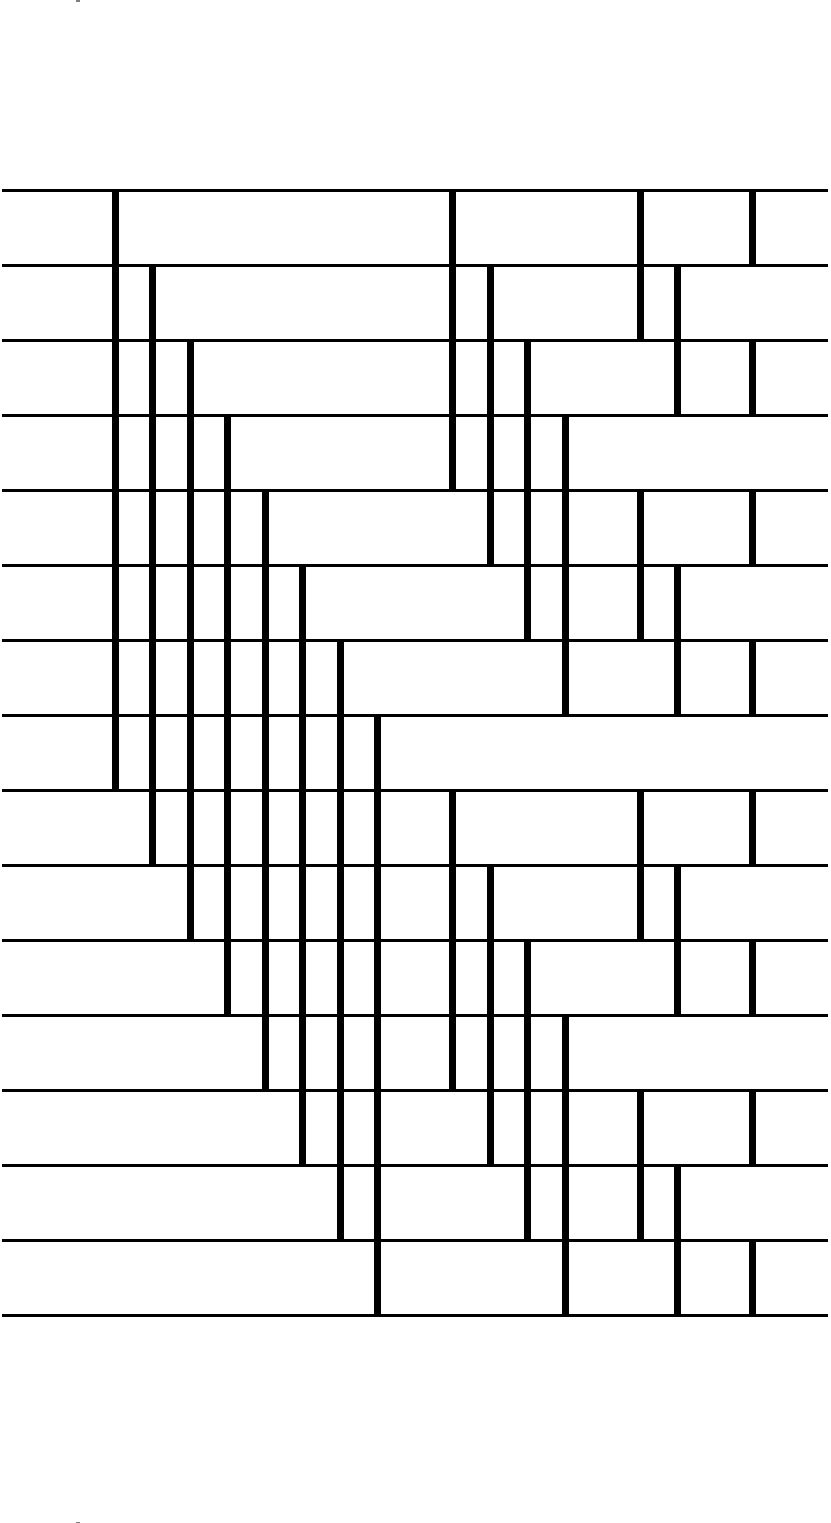
\includegraphics[scale=0.25]{./expressive/bitonic}
\caption{A diagram of a 16 input bitonic merging network, using
a style that is standard in the literature. Note
that in each stage containing 8 min/max or comparator components, all
8 operate on independent parts of the input and so can proceed in parallel.
}
\label{fig:bitonicMerger}
\end{figure}

We introduce a combinator {\tt ilv1}, for {\em interleave}, that captures this pattern.
{\tt ilv1 i f g} applies {\tt f} to elements {\small $2^i$} apart,
producing the output at the lower of the two input indices; it applies {\tt g}
to the same pairs of elements, producing the output on the upper index.
Defining {\tt stage i} to be {\tt ilv1 i min max},
the four stages in the diagram are simply
{\tt stage} applied to{\small  $3$, $2$ $1$} and {\small $0$}.
The definition of {\tt ilv1} makes use of the fact that
flipping the bit $i$ of an index (using
the function {\tt flipBit}) gives the index of the element
that will be combined with it using the functions{\tt f} and {\tt g}.
The decision about whether to apply {\tt f} or {\tt g} is made
by looking at the value of bit $i$.
As we shall see, the use of the Obsidian {\tt ifThenElse}
produces conditionals in the resulting CUDA.
\begin{codesize}
\begin{verbatim}
lowBit :: Int -> UWordE -> Exp Bool
lowBit i ix = (ix .&. bit i) ==* 0

flipBit :: Bits a => Int -> a -> a
flipBit = flip complementBit

ilv1 :: Choice a => 
        Int -> (b -> b-> a) -> (b -> b -> a) -> 
        Array b -> Array a
ilv1 i f g arr = Array ixf (len arr)
  where
    ixf ix = let l = arr ! ix
                 r = arr ! newix
                 newix = flipBit i ix
             in (ifThenElse (lowBit i ix) (f l r) (g l r))
\end{verbatim}
\end{codesize}
\noindent
Expressing {\tt ilv1} using bit-flipping may seem strange, but it has
the advantage that it actually applies the desired pattern of
computation repeatedly over larger input arrays.
Now, for {\small $2^n$} inputs, a Haskell list containing the $n$ calls
of this interleave combinator are built:
\begin{codesize}
\begin{verbatim}
bmerge :: Int -> [Array IntE -> Array IntE]
bmerge n = [istage (n-i) | i <- [1..n]]
  where istage i = ilv1 i min max
\end{verbatim}
\end{codesize}
\noindent
Finally, the {\tt compose} function makes each element of the list
into a kernel (using {\tt map pure}) and places a {\tt sync} between
each kernel (using {\tt composeS}).
\begin{codesize}
\begin{verbatim}
compose :: (Scalar a) => 
           [Array (Exp a) -> Array (Exp a)] 
           -> Array (Exp a) -> Kernel (Array (Exp a))
compose = composeS . map pure

runm k = putStrLn$ CUDA.genKernel "bitonicMerge" 
         (compose (bmerge k)) (namedArray "inp" (2^k))
\end{verbatim}
\end{codesize}
\noindent
Note that {\tt bmerge k} works on inputs of length {\small }$2^{k+j}$, for $j > 0$, applying the merger to sub-sequences of length {\small $2^k$}.
The CUDA code for {\tt bmerge 4} on $16$ inputs
(with some newlines inserted) is
\begin{codesize}
\begin{verbatim}
*Main> runm 4
__global__ void bitonicMerge(int *input0,int *result0){
  unsigned int tid = threadIdx.x;
  unsigned int bid = blockIdx.x;
  extern __shared__ unsigned char sbase[];
  (( int *)sbase)[tid] 
     = ((tid&8)==0) 
      ? min(input0[((bid*16)+tid)],input0[((bid*16)+(tid^8))]) 
      : max(input0[((bid*16)+tid)],input0[((bid*16)+(tid^8))]);
  __syncthreads();
  (( int *)(sbase + 64))[tid] 
     = ((tid&4)==0) 
      ? min((( int *)sbase)[tid],(( int *)sbase)[(tid^4)]) 
      : max((( int *)sbase)[tid],(( int *)sbase)[(tid^4)]);
  __syncthreads();
  (( int *)sbase)[tid] 
     = ((tid&2)==0) 
      ? min((( int *)(sbase+64))[tid],(( int *)(sbase+64))[(tid^2)]) 
      : max((( int *)(sbase+64))[tid],(( int *)(sbase+64))[(tid^2)]);
  __syncthreads();
  (( int *)(sbase + 64))[tid] 
     = ((tid&1)==0) 
      ? min((( int *)sbase)[tid],(( int *)sbase)[(tid^1)]) 
      : max((( int *)sbase)[tid],(( int *)sbase)[(tid^1)]);
  __syncthreads();
  result0[((bid*16)+tid)] = (( int *)(sbase+64))[tid];
\end{verbatim}
\end{codesize}

%% ** TODO Note that bmerge k not only works on inputs of length $2^{k+j}$,
%% for $j > 0$, applying the merger to sub-sequences of length $2^k$.

\subsection{Modifying the bitonic merger}


The bitonic merger for which we have just generated a kernel is known
to sort so-called bitonic sequences, which include sequences whose first
half is sorted in one direction and whose second half is sorted in the other
direction. This fact can be used to build the well-known bitonic sorting
network. However, a GPU implementation typically needs to check, for each comparator,
whether or not it should sort upwards or downwards, see for instance
the simple CUDA implementation shown in Appendix A.
We choose here to modify the merger so that it sorts two concatenated
sequences that are sorted in the {\em same} direction.
We do this by using a well-known trick, reversing half of the input to the merger. It turns out that
we can also reverse the same half of the output of the first stage of
the network, without affecting overall behaviour.
The resulting network, {\tt tmerge}, shown in Figure~\ref{fig:mixedMerger},
encourages us to develop a new combinator to describe the characteristic
V-shaped pattern that results in the first stage.
The combinator is modelled on {\tt ilv1}. The only difference
is that the ``partner'' of an index is found not by flipping bit $i$, but
by flipping bits $0$ to $i$, using function {\tt flipLSBsTo}. The implementation
of {\tt vee1} is got from that for {\tt ilv1} by replacing the call of
{\tt flipBit} by one of {\tt flipLSBsTo} (and we could also have chosen
to make a more generic function that is parameterised on this {\em partner} function).
\begin{codesize}
\begin{verbatim}
flipLSBsTo :: Int -> UWordE -> UWordE
flipLSBsTo i = (`xor` (oneBits (i+1)))

vee1 :: Choice a => 
        Int -> (b -> b-> a) -> (b -> b -> a) -> 
        Array b -> Array a
vee1 i f g arr = Array ixf (len arr)
  where
    ixf ix = let l = arr ! ix
                 r = arr ! newix
                 newix = flipLSBsTo i ix
             in (ifThenElse (lowBit i ix) (f l r) (g l r))
\end{verbatim}
\end{codesize}



\begin{figure}
\centering
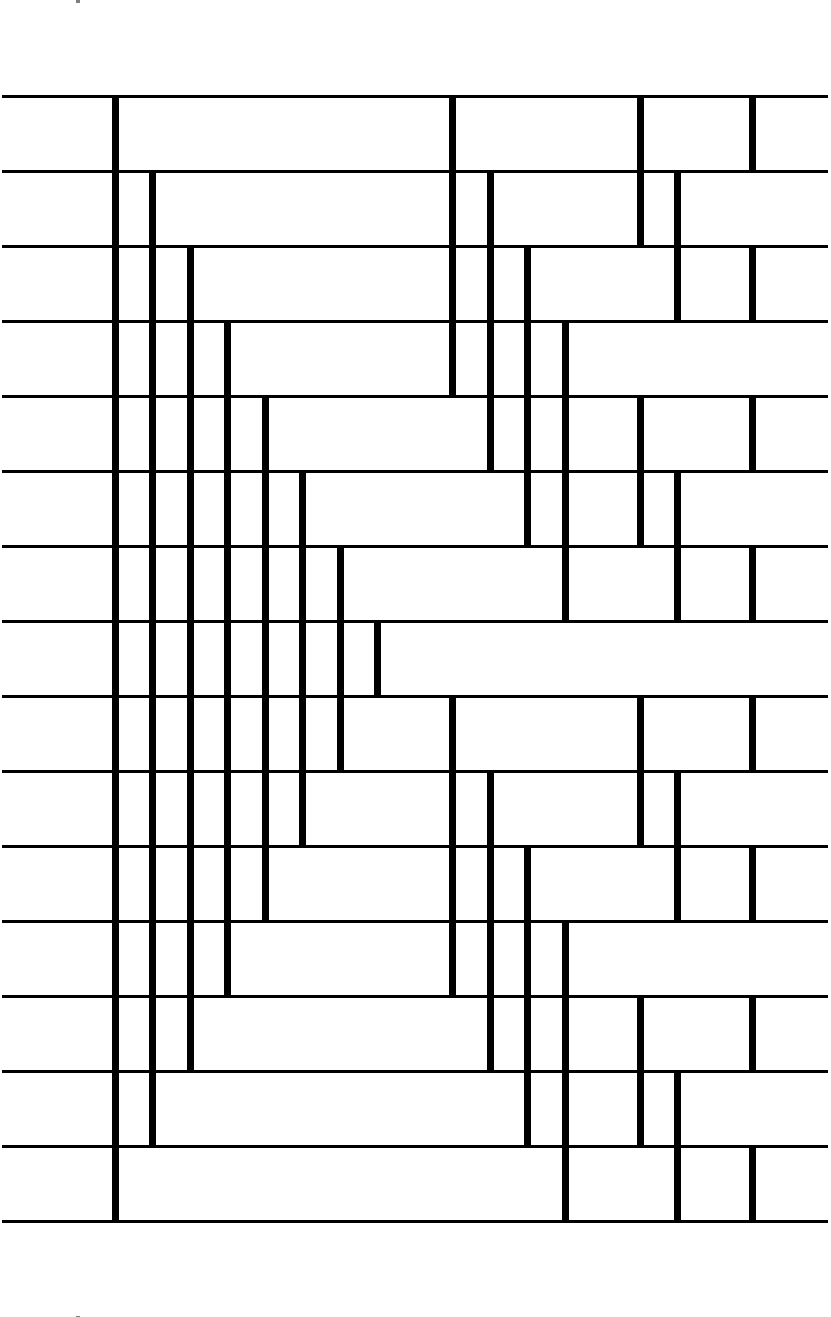
\includegraphics[scale=0.25]{./expressive/mixed}
\caption{16 input merging network, {\em tmerge}. The first stage
is made with a new combinator that we call vee, while
the remaining stages are as in the bitonic merger.
This network sorts an input that consists of two half-sized
sorted sequences, giving the opportunity to build a tree-shaped
sorting network.}
\label{fig:mixedMerger}
\end{figure}

\begin{codesize}
\begin{verbatim}
tmerge :: Int -> [Array IntE -> Array IntE]
tmerge n = vstage (n-1): [istage (n-i) | i <- [2..n]]
  where
    vstage i = vee1 i min max 
    istage i = ilv1 i min max
\end{verbatim}
\end{codesize}

Now that we have a merger that sorts sub-sequences containing two concatenated sorted sequences, it
is easy to make a tree of them.
The list of kernels to be composed now becomes
\begin{codesize}
\begin{verbatim}
tsort1 :: Int -> [Array IntE -> Array IntE]
tsort1 n = concat [tmerge i | i <- [1..n]]
\end{verbatim}
\end{codesize}
\noindent
The resulting sorting network is shown in Figure~\ref{fig:mixedsorter}.


\begin{figure}
\centering
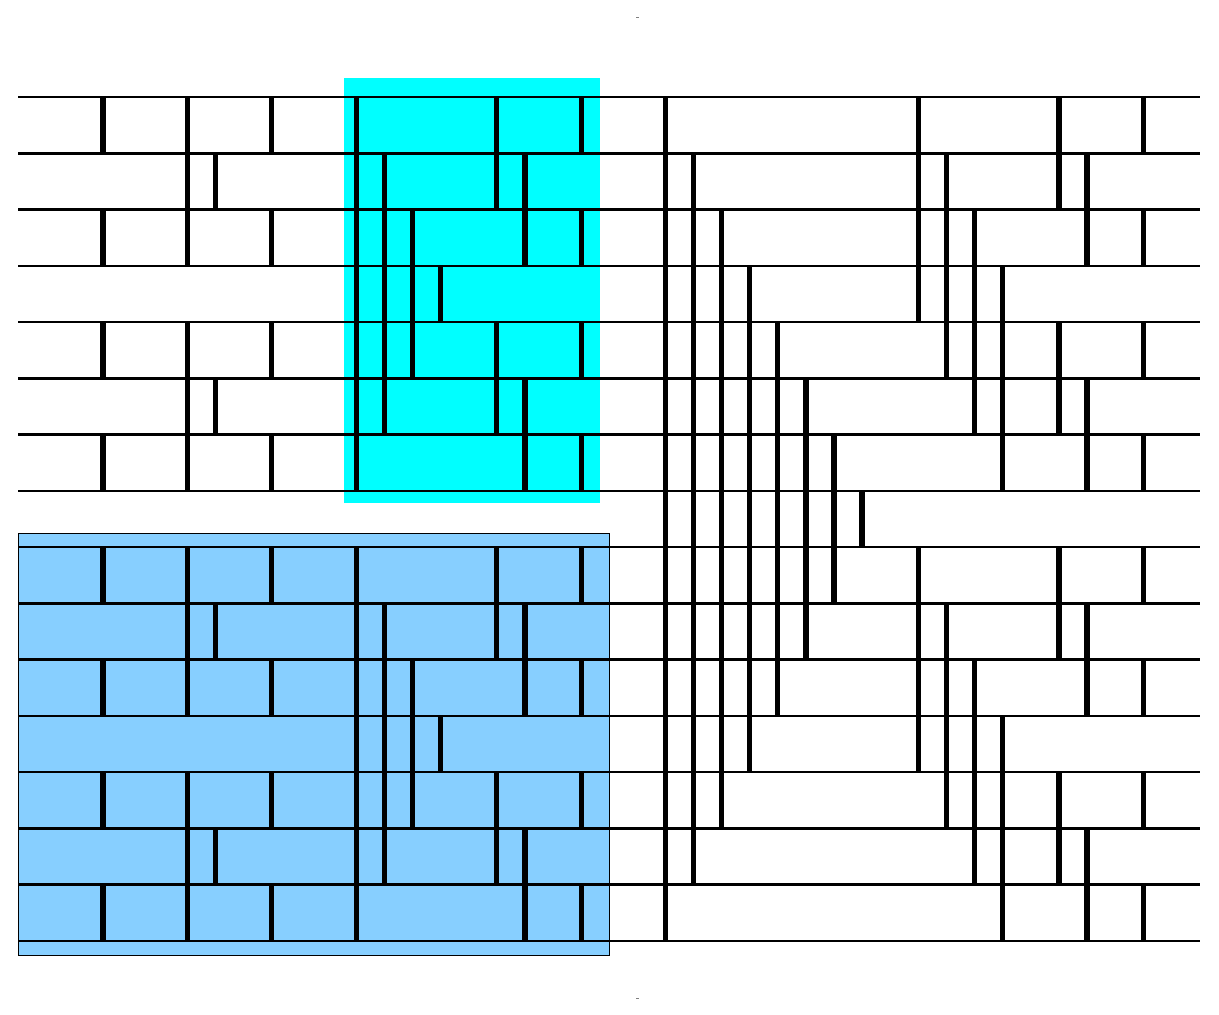
\includegraphics[scale=0.33]{./expressive/mmixedsorter}
\caption{A 16-input sorter made from a tree of {\em tmerge} mergers. 8 2-input mergers
feed 4 4-input mergers, followed  by 2 8-input and one 16-input merger.
A sorter on 8 inputs is shaded, as is a merger on 8 inputs, above it. 
}
\label{fig:mixedsorter}
\end{figure}
\noindent
The following call writes the resulting CUDA to file {\tt tsort1.cu}
and this is the first {\em generated} CUDA kernel whose performance is measured in section~\ref{sec:benchmarks}.

\begin{codesize}
\begin{verbatim}
runs1 k
  = writeFile "tsort1.cu" $ CUDA.genKernel "tsort1" 
      (compose (tsort1 k)) (namedArray "inp" (2^k))
\end{verbatim}
\end{codesize}

The generated code
% for $8$ inputs is shown in Appendix A. It 
uses
one thread per array element (just as the {\tt bitonicMerge}
kernel shown above did). The next step is to move to using Push as
well as Pull arays, so as to be able to generate more efficient code
from essentially the same sorter construction.

\subsection{New combinator implementations using Push arrays}

%% ** TODO make code for ilv2 more comprehensible :)

It is in combining the results of the {\tt f} and {\tt g} functions
that we run into difficulty using just Pull arrays.
Earlier, we saw how to use Push arrays to implement {\tt concP},
which concatenates two arrays.
Here, we use exactly the same approach to make a new version of
the {\em interleave} combinator. The results of applying
the {\tt f}s and {\tt gs} are combined into a Push array, in the right
order.
\pagebreak
%% ** TODO More explanation needed.
\begin{codesize}
\begin{verbatim}
ixMap :: (UWordE -> UWordE) -> ArrayP a -> ArrayP a 
ixMap f (ArrayP p n) = ArrayP (ixMap' f p) n

ixMap' :: (UWordE -> UWordE) 
         -> P (UWordE, a)
         -> P (UWordE, a) 
ixMap' f p = \g -> p (\(i,a) -> g (f i,a))

insertZero :: Int -> UWordE -> UWordE
insertZero 0 a = a `shiftL` 1
insertZero i a 
  = a + (a .&. fromIntegral (complement (oneBits i :: Word32)))

ilv2 :: Choice b => 
        Int -> (a -> a -> b) -> (a -> a -> b) -> 
        Array a -> ArrayP b
ilv2 i f g (Array ixf n) 
   = ArrayP (\k -> app a5 k *>* app a6 k) n
  where
    n2 = n `div` 2
    a1 = Array (ixf . left) (n-n2)
    a2 = Array (ixf . right) n2
    a3 = zipWith f a1 a2
    a4 = zipWith g a1 a2
    a5 = ixMap left (push a3)
    a6 = ixMap right (push a4)
    left = insertZero i
    right = flipBit i  . left
    app (ArrayP f _) a = f a
\end{verbatim}
\end{codesize}
\noindent
This new combinator can now replace {\tt ilv1} in the bitonic
merger, giving a kernel that runs considerably faster. We will use
that kernel to build a large sorter later.

The implemenation of {\tt vee2} is almost identical to
that of {\tt ilv2}, with {\tt flipBit i}
replaced by {\tt flipLSBsTo} as before (so that, again, one would in
fact make a more generic function for building such combinators).
Now, we just need to replace the {\tt ilv1} and {\tt vee1} combinators
in the tree sorter with {\tt ilv2} and {\tt vee2} , to get a verrsion that uses half as many threads:
\begin{codesize}
\begin{verbatim}
tmerge2 :: Int -> [Array IntE -> ArrayP IntE]
tmerge2 n = vstage (n-1) : [ istage (n-i) | i <- [2..n]]
  where
    vstage i = vee2 i min max
    istage i = ilv2 i min max


tsort2 :: Int -> [Array IntE -> ArrayP IntE]
tsort2 n = concat [tmerge2 i | i <- [1..n]]
\end{verbatim}
\end{codesize}
As we shall see in section~\ref{sec:benchmarks}, the resulting code
is significantly faster. This is because it uses one thread per two array elements,
and the code no longer contains any conditionals.

In order to go faster still, we resort to building a different sorting network, of
exactly the same size as the bitonic sorter, but based instead on the balanced period merger of Dowd et al~\cite{PeriodicBalanced}.
This involves the introduction of one new combinator that can be seen as a mixture
of the {\tt ilv} and {\tt vee} combinators already introduced.

\subsection{A sorter built from the balanced periodic merger}
First, we note that the balanced periodic merger contains multiple
uses of the now familiar vee-shaped pattern, see Figure~\ref{fig:periodicMerger}.
\begin{figure}
\centering
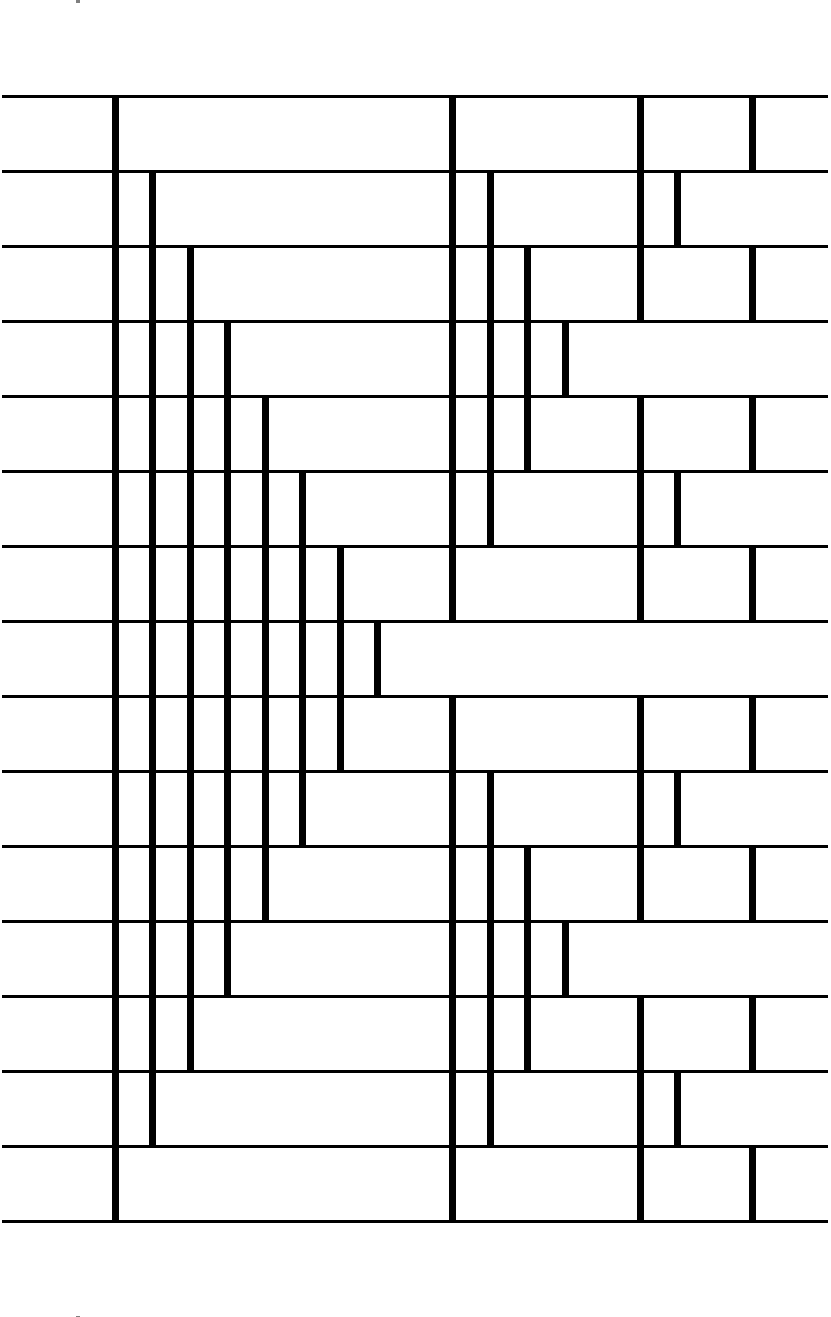
\includegraphics[scale=0.25]{./expressive/balanced}
\caption{16 input periodic balanced merging network}
\label{fig:periodicMerger}
\end{figure}

\begin{codesize}
\begin{verbatim}
bpmerge2 :: Int -> [Array IntE -> ArrayP IntE]
bpmerge2 n = [vstage (n-i) | i <- [1..n]]
  where vstage i = vee2 i min max
\end{verbatim}
\end{codesize}

Now Dowd et al proved that the balanced periodic merger sorts two {\em interleaved} sorted sequences. So, taking an iterative view of the resulting sorter,
we want to build a tree of mergers as before, but the smaller mergers should
be interleaved, rather than operating on adjacent sub-sequences.
There should be one merger on the right hand end of the network; left of
that, there should be two mergers that operate on the odd and even elements,
and each of them should in turn be fed by two interleaved mergers, and so.
The sorter is illustrated, for $16$ inputs in Figure~\ref{fig:vsorter}.
Just to the left of the final balanced merger, one of the two interleaved
mergers is shown using dotted lines. It operates on a completely different set of inputs from the other 8-input merger in the same part of the tree.

\begin{figure*}
\centering
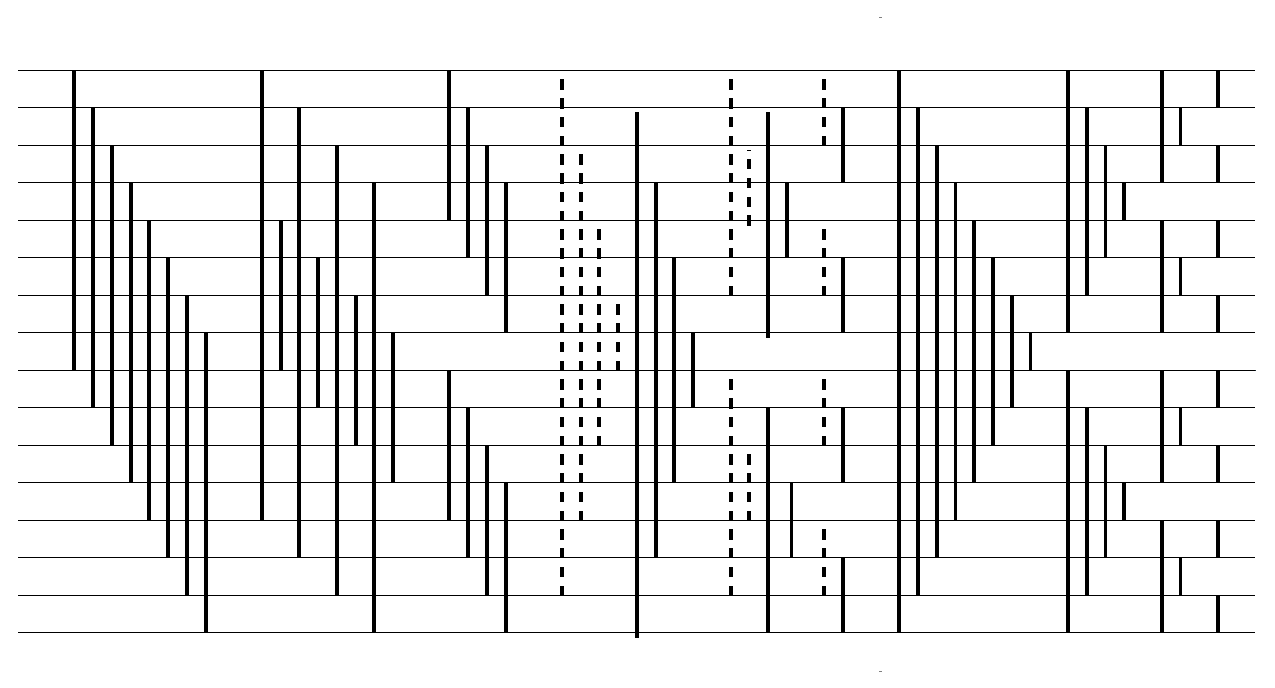
\includegraphics[scale=0.5]{./expressive/vsorter}
\caption{A sorter based on the idea that the periodic
balanced merger network sorts two interleaved sorted sequences.
It consists of two half-sized sorters, one working on the
odd elements of the input and one on the even, followed by
the balanced merger. The diagram indicates using dotted lines the
balanced merger that is the final (rightmost) part of
one of the half-size sorters.}
\label{fig:vsorter}
\end{figure*}

The most straightforward way to give an iterative description of
this sorter is
to introduce a new combinator that is a combination of
{\tt ilv} and {\tt vee}.
The only thing that we need to change is the {\em partner} function.
This time we will flip not the least significant bits from position $0$ to
position $i$ but from position $i$ to $i+j$.

\begin{codesize}
\begin{verbatim}
-- flip bits from position i to position i+j inclusive
flipBitsFrom :: Bits a => Int -> Int -> a -> a
flipBitsFrom i j a = a `xor` (fromIntegral mask)
  where
    mask = (oneBits (j + 1):: Word32) `shiftL` i

ilvVee1 :: Choice a => 
           Int -> Int -> 
           (b -> b-> a) -> (b -> b -> a) -> 
           Array b -> Array a
ilvVee1 i j f g arr = Array ixf (len arr)
  where
    ixf ix = let l = arr ! ix
                 r = arr ! newix
                 newix = flipBitsFrom i j ix
             in (ifThenElse (lowBit (i+j) ix) (f l r) (g l r))
\end{verbatim}
\end{codesize}

\begin{codesize}
\begin{verbatim}
ilvVee2 :: Choice b => Int -> Int -> 
           (a -> a -> b) -> (a -> a -> b) -> 
           Array a -> ArrayP b
ilvVee2 i j f g (Array ixf n) 
  = ArrayP (\k -> app a5 k *>* app a6 k) n
  where
    n2 = n `div` 2
    a1 = Array (ixf . left) (n-n2)
    a2 = Array (ixf . right) n2
    a3 = zipWith f a1 a2
    a4 = zipWith g a1 a2
    a5 = ixMap left (push a3)
    a6 = ixMap right (push a4)
    left = insertZero (i+j)
    right = flipBitsFrom i j . left
    app (ArrayP f _) a = f a
\end{verbatim}
\end{codesize}

For both variants of the combinator, we simply add to the {\tt ilv} definitions
a new {\tt Int} parameter, {\tt j}, and replace {\tt flipBit i} by {\tt flipBitsFrom i j}. We also insert the zero bit (when calculating the left index)
at position {\tt i + j} rather than just at position {\tt i}.
{\tt ilvVee} is a generalisation of both {\tt ilv} and {\tt vee}.
{\tt ilvVee i 0} has the same behaviour as {\tt ilv i}, and {\tt ilvVee 0 (j-1)}
is the same as {\tt vee j}. The {\tt i} parameter controls the degree
of interleaving, and the {\tt j} parameter controls the size of
the vee-shaped blocks.

For $16$ inputs, the parameters
to {\tt ilvVee} that describe the periodic merger on the right of the construction
are $i=0$ (for no interleaving) paired with $3$, $2$, $1$ and $0$
for the decreasing size of the vee-shaped blocks.
Next, to the left, the mergers are interleaved ($i=1$) and there are three
stages with
vee-shaped blocks of decreasing size ($j = 2, 1, 0$), see Figure~\ref{fig:vsorter}.
The following code gives an iterative description of the construction
for {\small $2^n$} inputs:


\begin{codesize}
\begin{verbatim}
vsort :: Int -> Array IntE -> Kernel (Array IntE)
vsort n = composeS . map pure $ [istage (n-i) (i-j) 
                                | i <- [1..n], j <- [1..i]]
  where istage i j = ilvVee2 i j min max
\end{verbatim}
\end{codesize}

\noindent
The resulting generated code uses one thread per
$2$ indices.

\subsection{Measuring performance of the generated kernels}\label{sec:benchmarks}
\begin{figure}
\begin{codesize}
\begin{verbatim}
  unsigned int arrayLength = 1 << LOG_L_SIZE;
  unsigned int diff = LOG_L_SIZE - LOG_S_SIZE;
  unsigned int blocks = arrayLength / S_SIZE;
  unsigned int threads = S_SIZE / 2;
  
  sortSmall<<<blocks, threads,4096>>>(din,din);
 
  for(int i = 0 ; i < diff ; i += 1){ 
    vSwap<<<blocks/2,threads*2,0>>>(din,din,(1<<i)*S_SIZE);
     
    for(int j = i-1; j >= 0; j -= 1)
      iSwap<<<blocks/2,threads*2,0>>>(din,din,(1<<j)*S_SIZE);
      
    bmergeSmall<<<blocks,threads,4096>>>(din,din);}
\end{verbatim}
\end{codesize}
\caption{CUDA code for our large sorter. {\tt sortSmall} and {\tt bmergeSmall}
are replaced by Obsidian-generated kernels in the experiments. {\tt vSwap} and {\tt iSwap} are handwritten CUDA kernels
that perform one column of compare and swap operations in the vee and ilv shapes respectively, and are
parameterised on the stride. (Our generated kernels have fixed input and output size.)}
\label{fig:CUDAsort}
\end{figure}
We have measured the performance of generated 512-input sorting and merging kernels by plugging them into a larger sorter written in CUDA.
The sorter has exactly the structure shown in Figure~\ref{fig:mixedsorter}.
Figure~\ref{fig:newmixedsorter} shows the location of smaller sorters and mergers, and of vSwap and iSwap kernels for $16$ inputs.
Larger sorters simply have more columns of mergers, each preceded by a vSwap and a number of iSwaps.
The overall structure of the resulting CUDA code is shown in Figure~\ref{fig:CUDAsort}.
Because {\tt iSwap} is used repeatedly, we also wrote kernels
corresponding to compositions of two and three of them (avoiding
memory accesses between the columns).
That is, we replaced the loop containing {\tt iSwap} above by
\pagebreak
\begin{codesize}
\begin{verbatim}
for(int j = i-1; j >= 0; j -= 3){ 
  if (j==0) 
    iSwap<<<blocks/2,threads*2,0>>>(din,din,(1<<j)*S_SIZE);
    else 
    {if (j==1) 
       iSwap2<<<blocks/4,threads*2,0>>>(din,din,(1<<j)*S_SIZE);
       else 
       iSwap3<<<blocks/8,threads*2,0>>>(din,din,(1<<j)*S_SIZE);}}
\end{verbatim}
\end{codesize}
\noindent
The Obsidian implementation and all code for examples in the paper are available at \url{http://www.cse.chalmers.se/~joels/expressive.html}.

\begin{figure}
\centering
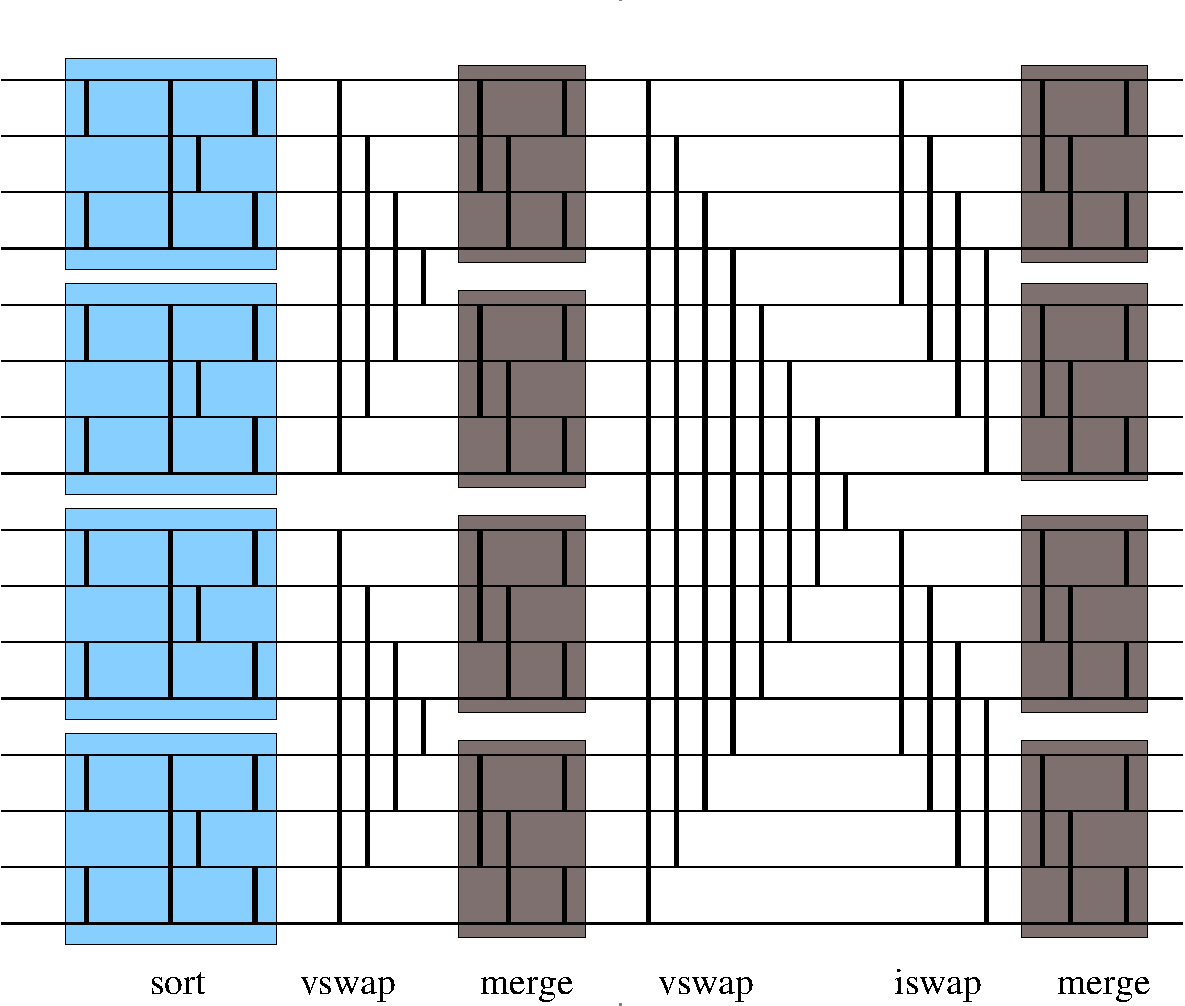
\includegraphics[scale=0.33]{./expressive/newmixedSorter}
\caption{
This diagram shows the tree-shaped sorting network that we saw earlier, but with 4 input sorting and merging kernels indicated. This is the structure of the network that we have used to implement large sorters, in which the small kernels having {\small $2^9 = 512$} inputs in all cases. For {\small $2^{24}$} inputs overall, the resulting sorter
has one column of small sorters and $24-9=15$ of small mergers.}
%% both ofs in the above sentence should remain :)
\label{fig:newmixedsorter}
\end{figure}

Table~\ref{fig:table} shows the performance figures for the large sorter
for $5$ different $512-$input small sorter kernels.
{\tt tsort1} is defined above, and is a variant of bitonic sort
that does not require {\tt if} statements to determine the direction
of sorting of pairs, as all comparison operations place the minimum at the
same index as the lower input.
{\tt tsort2} is the same construction, but built with the combinators {\tt ilv2}
and {\tt vee2} that result in the use of one thread per two indices.
{\tt vsort}, the fastest kernel, uses a generalisation of those
two combinators, and again uses one thread per two indices.
{\tt vsort1} is the same construction as {\tt vsort}, but with {\tt ilvVee2} replaced
by {\tt ilvVee1}, and so using one thread per index.
As a reference small kernel implementation, we include a simple hand-coded bitonic sort
that uses one thread per index (see code in Appendix).
None of the kernels has been subject to optimisations related to warp size.

% table 


\begin{table}
\begin{center}
  \begin{tabular}{| l | r | r | r | r | r | r | }
    \hline
        k                             &  $20$ &  $21$ & $22$& $23$ & $24$ & $24$(CPU)  \\ \hline
    bitonic(CUDA)(512)                &  5 & 12 & 25 & 54 & 117 & 2741   \\      
    tsort1(512)                       &  4 & 10 & 22 & 47 & 102 & 2742    \\
    tsort2(256)                       &  4 & 9 & 23 & 45 & 98 & 2741     \\ 
    vsort1(512)                       &  4 & 10 & 21 & 47 & 102 & 2747    \\ 
    vsort(256)                        &  4 & 9 & 20 & 44 & 96 & 2783    \\ 
    \hline
  \end{tabular}
\end{center}
\label{tab:expressive-table1}
\caption{Sorting time (ms) for $2^k$ inputs, $20 \leq k \leq 24$.  The GPU used is an NVIDIA GTX480.
Each line shows the result using a particular small $512$ input sort kernel with the
indicated number of threads as {\tt sortSmall} in the CUDA code above. The small merge kernel used
is our generated {\tt bmerge2}, with two indices per thread and $512$ inputs. Memory transfer time (GPU-CPU)
is not shown. In the $2^{24}$ input case using {\tt vsort}, the total sorting time, including
memory transfers was 141 ms.
The rightmost column shows the time taken for the C quicksort function {\tt qsort}, compiled with
{\tt gcc -O3}, to sort the same inputs as those sorted on the GPU on an i7-920 2.8GHz CPU.
} 
\end{table}




%% bitonic 30203
%% 


We also recorded the GPU time spent in the calls to the small sorters alone (using the NVIDIA CUDA Visual profiler), see Table~\ref{tab:table2}.
The {\tt tsort1} and {\tt vsort1} kernels, which are built using only pull arrays, 
(and which have one index per thread in the generated code) are
noticeably slower than those that have two indices per thread.
The generation of the latter kernels is made possible by the introduction of 
push arrays.

% table 


\begin{table}
\begin{center}
  \begin{tabular}{| l | r | r |   }

    \hline
                              & time & percent \\ \hline
    bitonic(CUDA)             & 30203 & 32.07\\
    tsort1                    & 15823 & 19.72  \\
    vsort1                       & 14955 & 18.76 \\ 
    tsort2                      & 11562 & 15.37    \\ 
    vsort                       & 9228 &  12.67 \\ 
    bitonic (NVIDIA SDK)        & 23815 & 6.55 \\
    \hline
  \end{tabular}
\end{center}
\label{tab:expressive-table2}
\caption{time: GPU time (in $\mu$s) spent in calls to small sorter kernels 
in the initial phase of the sorter for $2^{24}$ inputs. percent: percentage 
of total GPU time spent in the small sort kernel.
The final line shows the numbers for the bitonic code (for large sorts) that 
is distributed with the the NVIDIA SDK. Its structure also starts with a phase 
of small sorting kernels. It takes 274 ms to sort $2^{24}$ key-value pairs on 
an NVIDIA GTX480 GPU. It could be sped up by using our {\tt vsort} kernel, 
and also by (hand) fusing single ``column'' kernels as we did with {\tt iSwap}, 
although the need to calculate directions of comparators in the bitonic network 
would complicate this. Our CUDA code is simpler because all comparators
point in the same direction in the sorter construction.
} 
\end{table}






%% bitonic 30203
%% tsort1 15823
%% tsort2 11562
%% vsort1 14955
%% vsort 9228


Although none of our generated kernels is optimised (for example with respect to warp size), 
their performance is, nevertheless, very good. We are working on automated warp size-related 
optimisations. It would also be interesting to explore the fusion of adjacent columns of 
comparators in the small kernels; omitting a {\tt sync} would cause this fusion to happen
but we also need to modify the threading behaviour (doubling the number of indices per thread).


%The final version of the paper will contain benchmarking against a highly optimised sorter kernel obtained from our colleagues in the computer graphics group at Chalmers. For now, we emphasise that the {\tt vsort} kernel is so fast that we expect it to compare favourably. Given the simplicity of its description in Obsidian, we feel that this is a good way to write fast kernels.
